%%%%%%%%%%%%%%%%%%%%%%%%%%%%%%%%%%%%%%%%%%%%%%%%%%%%%%%%%%%%%%%%%%%%%%
% LaTeX Template: Designer's CV
%
% Source: http://www.howtotex.com
% 
% Feel free to distribute this example, but please keep the referral
% to HowToTeX.com
% 
% Date: March 2012
%
% Modified by Lim Lian Tze to support multiple pages using fix provided at
% http://www.howtotex.com/templates/creating-a-designers-cv-in-latex/
% Date: November 2014
%%%%%%%%%%%%%%%%%%%%%%%%%%%%%%%%%%%%%%%%%%%%%%%%%%%%%%%%%%%%%%%%%%%%%%
% How to use writeLaTeX: 
%
% You edit the source code here on the left, and the preview on the
% right shows you the result within a few seconds.
%
% Bookmark this page and share the URL with your co-authors. They can
% edit at the same time!
%
% You can upload figures, bibliographies, custom classes and
% styles using the files menu.
%
% If you're new to LaTeX, the wikibook is a great place to start:
% http://en.wikibooks.org/wiki/LaTeX
%
%%%%%%%%%%%%%%%%%%%%%%%%%%%%%%%%%%%%%%%%%%%%%%%%%%%%%%%%%%%%%%%%%%%%%%

%%%%%%%%%%%%%%%%%%%%%%%%%%%%%%%%%%%%%
% Document properties and packages
%%%%%%%%%%%%%%%%%%%%%%%%%%%%%%%%%%%%%
\documentclass[a4paper,12pt,final]{memoir}

% misc
\renewcommand{\familydefault}{bch}	% font
\pagestyle{empty}					% no pagenumbering
\setlength{\parindent}{0pt}			% no paragraph indentation


% required packages (add your own)
\usepackage{flowfram}										% column layout
\usepackage[top=1cm,left=1cm,right=1cm,bottom=1cm]{geometry}% margins
\usepackage{graphicx}										% figures
\usepackage{url}											% URLs
\usepackage[usenames,dvipsnames]{xcolor}					% color
\usepackage{multicol}										% columns env.
	\setlength{\multicolsep}{0pt}
\usepackage{paralist}										% compact lists
\usepackage{tikz}

%%%%%%%%%%%%%%%%%%%%%%%%%%%%%%%%%%%%%
% Create column layout
%%%%%%%%%%%%%%%%%%%%%%%%%%%%%%%%%%%%%
% define length commands
\setlength{\vcolumnsep}{\baselineskip}
\setlength{\columnsep}{\vcolumnsep}

% left frame
\newflowframe{0.3\textwidth}{\textheight}{0pt}{0pt}[left]
	\newlength{\LeftMainSep}
	\setlength{\LeftMainSep}{0.22\textwidth}
	\addtolength{\LeftMainSep}{1\columnsep}
 
% small static frame for the vertical line
\newstaticframe{1.5pt}{\textheight}{\LeftMainSep}{0pt}
 
% content of the static frame
\begin{staticcontents}{1}
\hfill
\tikz{%
	\draw[loosely dotted,color=RoyalBlue,line width=1.5pt,yshift=0]
	(0,0) -- (0,\textheight);}%
\hfill\mbox{}
\end{staticcontents}
 
% right frame
\addtolength{\LeftMainSep}{1.5pt}
\addtolength{\LeftMainSep}{1\columnsep}
\newflowframe{0.7\textwidth}{\textheight}{\LeftMainSep}{0pt}[main01]


%%%%%%%%%%%%%%%%%%%%%%%%%%%%%%%%%%%%%
% define macros (for convenience)
%%%%%%%%%%%%%%%%%%%%%%%%%%%%%%%%%%%%%
\newcommand{\Sep}{\vspace{1.5em}}
\newcommand{\SmallSep}{\vspace{0.5em}}

\newenvironment{AboutMe}
	{\ignorespaces\textbf{\color{RoyalBlue} About me}}
	{\Sep\ignorespacesafterend}
	
\newcommand{\CVSection}[1]
	{\Large\textbf{#1}\par
	\SmallSep\normalsize\normalfont}

\newcommand{\CVItem}[1]
	{\textbf{\color{RoyalBlue} #1}}


%%%%%%%%%%%%%%%%%%%%%%%%%%%%%%%%%%%%%
% Begin document
%%%%%%%%%%%%%%%%%%%%%%%%%%%%%%%%%%%%%
\begin{document}

% Left frame
%%%%%%%%%%%%%%%%%%%%
%
% Upload your own photo using the files menu
\begin{figure}
	%\hfill
	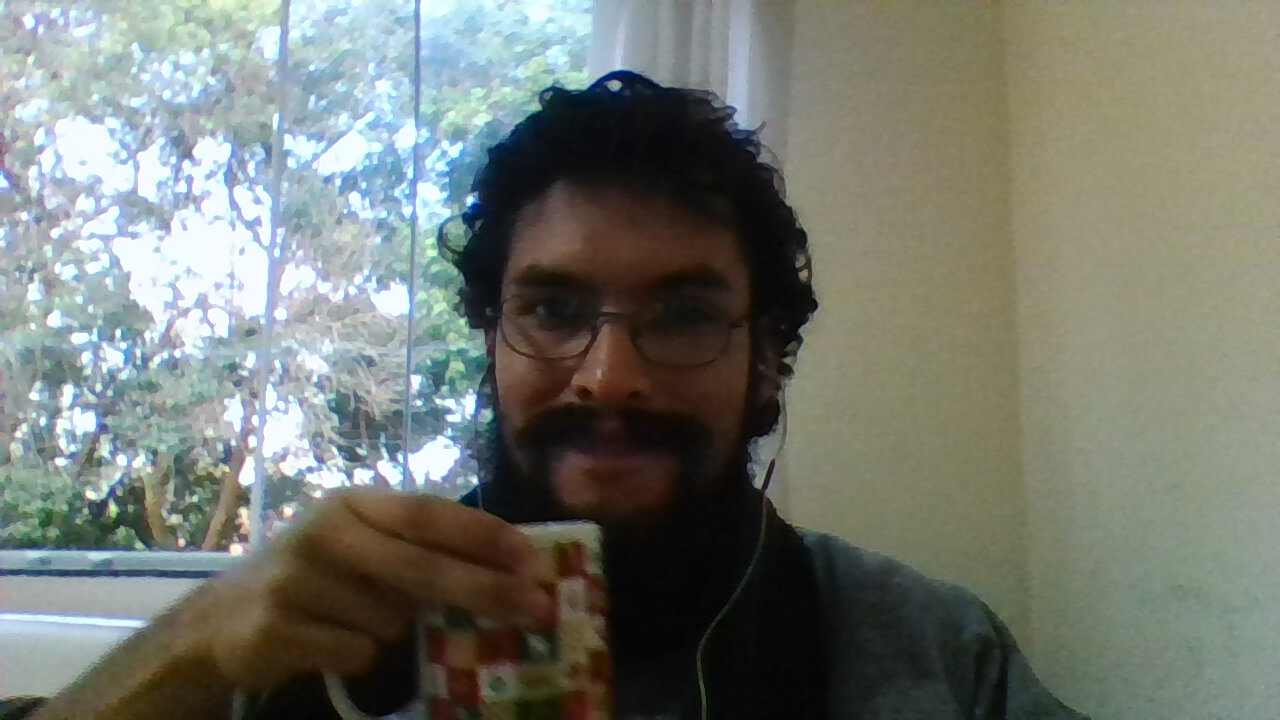
\includegraphics[width=0.75\columnwidth]{my-pic.jpg}
	\vspace{-2cm}
\end{figure}

\begin{flushleft}\small
    \vspace{10mm}
    \textbf{Contact Details}\\
    \vspace{1mm}
	Gabriel D\'iaz Iturry\\
%	\vspace{1mm}
%	- \\
	\vspace{1mm}
    
\includegraphics[width=0.07\columnwidth]{gmail_icon.png} gabriel.diaz.iturry\\
    \vspace{1mm}
%    
\includegraphics[width=0.08\columnwidth]{usp_icon.png} gditurry@if.usp.br \\
    %
\includegraphics[width=0.07\columnwidth]{cellphone_icon.png} -\\	
%	\vspace{4mm}
%	\textbf{Work Address}\\
%	\vspace{1mm}
%	-\\
%	\vspace{1mm}
%	- \\
%	\vspace{1mm}
%	-\\
%	\vspace{1mm}
%	-\\
%	\vspace{4mm}
%	\textbf{Personal Address}\\
%	\vspace{1mm}
%	- \\
%	\vspace{1mm}
%	- \\
%	\vspace{1mm}
%	- \\
%	\vspace{1mm}
%	-\\
%	\vspace{4mm}
%	\textbf{Details and Publications}\\
%	\vspace{1mm}
%	Curriculo Lattes \\
%	\vspace{1mm}
%	- \\
%	\vspace{1mm}
    
\includegraphics[width=0.07\columnwidth]{in_icon.png} /in/gabriel-diaz-iturry \\
    \vspace{1mm}
    
\includegraphics[width=0.07\columnwidth]{git.jpeg} /gabo-di \\
    \vspace{1mm}
    \vspace{4mm}
	\textbf{Languages}\\
	\vspace{1mm}
	Spanish: Mother tongue\\
	\vspace{1mm}
	English: Advanced\\
	\vspace{1mm}
	Portuguese: Fluent\\
	\vspace{1mm}
	Esperanto: Intermediate
\end{flushleft}\normalsize


\framebreak



% Right frame
%%%%%%%%%%%%%%%%%%%%
\Huge\bfseries {\color{RoyalBlue} D\'iaz Gabriel Iturry} \\
\Large\bfseries Physicist - Data Scientist\\

\normalsize\normalfont
\vspace{-10pt} 
% About me
\begin{AboutMe}
Since 2012, I have worked as a scientific researcher in the area of Nonlinear Dynamics. During this period, I have acquired advanced mathematical knowledge and learned several computational skills concerning data analysis. This involves the manipulation and interpretation of data and the use of statistical tools to compare data to models. I currently work for CAP4GI, writing a Julia repository for ecological/agricultural research.
\end{AboutMe}

\vspace{-15pt} 
% Experience
\CVSection{Experience}

\CVItem{April 2024 - Present}\\
{\small Julia/Fortran Developer:}
\begin{footnotesize}
\begin{itemize}
\item Open source Julia repository for ecological research in the group CAP4GI.
\item Use of Fortran code AquaCrop from FAO.
\end{itemize}
\end{footnotesize}
\SmallSep


\CVItem{Jan 2023 - April 2024t}\\
{\small Independent Researcher:}
\begin{footnotesize}
\begin{itemize}
\item Research in areas of Time Series analysis using Artificial Intelligence and Data Driven Modeling. 
\item Web developer, in charge of integrating the AI code with the Web page.
\end{itemize}
\end{footnotesize}
\SmallSep

\CVItem{May 2021 - Apr 2023}\\
{\small Data Scientist, Physicist:}
\begin{footnotesize}
\begin{itemize}
\item Reproduce state-of-the-art reasearch.
\item Deliver the models in a clear and robust interfarce for user consumption.
\item Optimization using Operations Research and Heuristics methods for several projects.
\end{itemize}
\end{footnotesize}
\SmallSep

\CVItem{Feb 2017 - Feb 2021}\\
\begin{small}
Researcher and Teaching Assistant,  Instituto de F\'{i}sica, Universidade de S\~{a}o Paulo 
(USP). S\~{a}o Paulo, Brazil. 
Research projects include: 
\end{small}
\begin{footnotesize}
\begin{itemize}
\item Anomalous Diffusion on Classical Systems.
\item Bifurcation Analysis.
\item Quantum to Classical transition.
\end{itemize}
\end{footnotesize}

\SmallSep


% Education
\CVSection{Education}
\CVItem{2017 - 2021}\\
\begin{small}
 Ph. D. in Physics, Universidade de S\~{a}o Paulo (USP).\\ 
S\~{a}o Paulo, Brazil.
 \end{small} 
\SmallSep

\CVItem{2015 - 2017}\\
\begin{small}
M. Sc. in Physics, Universidade Estadual de S\~{a}o Paulo (UNESP)\\
S\~{a}o Paulo, Brazil.
\end{small}
\SmallSep

%\CVItem{2009 - 2014}\\
%\begin{small}
%Bachelor in Physics, Universidad Mayor de San Sim\'{o}n (UMSS).\\
%Cochabamba, Bolivia.
%\end{small}


\CVSection{Skills}

% Skills

\CVItem{Technical}\\
{\small Scientific Research, Scientific Computing, Simulations, Neural Networks, Machine Learning\\}
\vspace{-10pt}
\SmallSep

\CVItem{Software Development}\\
\begin{small}
Python, R, Julia, Fortran, Golang, Mathematica, MatLab.\\
PyTorch, Tensorflow, Keras, sklearn, XGBoost, CatBoost.\\
\end{small}


% References

%\CVSection{References}

%References upon request.

%%%%%%%%%%%%%%%%%%%%%%%%%%%%%%%%%%%%%
% End document
%%%%%%%%%%%%%%%%%%%%%%%%%%%%%%%%%%%%%
\end{document}